\documentclass[uplatex,dvipdfmx]{jsarticle}

\input{"preamble.tex"}

\title{物質科学のための群論入門}
\author{ガオゾウ}

\begin{document}
\maketitle
\section{導入:物質の対称性と群論}
現実の物質を対象とする物質科学は、理論的な解析が非常に困難なことが多いです。その理由としては例えば、ほとんどの場合に自由度が非常に多いことや、相互作用を考慮しなくてはならないことが挙げられます。このような系では、理論的に厳密な解析をするのは困難であるため、しばしば大胆な近似を行う必要があります。

そんな物質の理論を構築するにあたり非常に重要となる一つの手がかりが、物質の持つ対称性です。対称性のもっとも簡単な例は「左右対称」でしょう。しばしば物質も「左右対称」を含む様々な対称性を持ちえます。実は、このような対称性を持つ・持たないという情報だけから物質の様々な性質を知ることができるのです。しかも、このような議論は、しばしば理論的に厳密に行うことができます。複雑な物質であっても、対称性は容易にわかることが多いので、これは非常に強力な手法です。

% 例えば、キラル分子が旋光性を持つ(光学活性である)というのは、まさに分子の持つ対称性から理解することができます。そのほか錯体分子の配位子場分裂や結晶場分裂は、その物質の持つ対称性の変化から生じるものです。
% また、固体物理学で最も基本的な理論であるバンド理論も物質の対称性に基づく理論の一つです。本来バンド理論は結晶中の電子の理論ですが、そこで出てくる「分散関係」という言葉がそのほかの様々な結晶中の粒子(フォノン、マグノン、etc.)にも用いられているのは、これらの理論は全て共通して結晶の持つ対称性を背景に持つからです。

% いろいろと例を挙げましたが、物理・化学と分野を問わず、物質科学において「対称性」が非常に基本的な考え方であることがわかっていただけたでしょうか。

このような対称性の議論をするにあたって基本的な道具となるのが、本記事のテーマである群論、特に群の表現論です。

本記事の基本的な流れは以下のようになります。まず、群の定義を簡単に述べた後、群の表現の定義を述べます。その後、群の表現に関する重要な定理をいくつか紹介します。その後、これらの定理を用いた実際の物質の解析例を紹介します。

前提知識としては、線形代数と量子力学の基本的な知識を仮定します。「シュレーディンガー方程式を解くということはハミルトニアンを対角化することだ」と言われて意味がわかれば大丈夫です。群論については、一応群の公理から話を始めるので、前提知識は原理的にはいりません。しかし、多少は触れたことがあった方が話は分かりやすいとは思います。

本記事ではあくまで物質の解析への応用を主眼とするので、定理の証明にはあまり踏み込みません。興味のある方は参考文献にも挙げている応用群論\cite{ouyougunron}などをご覧ください。

%  対称性のもっとも簡単な例の一つは正方形です。正方形は様々な対称性を持っています。例えば、正方形は図1(a)のように、中心線に関して折りたたむときれいに重なります。つまり左右対称です。このことは、

 

% また、図1(b)のように90°(1/4回転)だけ正方形を回転しても、元の形に戻ります。このような対称性を4回対称性と呼びます。正方形は同時に、2回対称性も持ちます。すなわち、180°(1/2回転)だけの回転に対しても、やはり元の形に戻ります。

\section{対称性と群論の概観}
\subsection{群の定義}
群とは、以下の四つの公理を満たす集合$G$と演算$\vdot$(積と呼ぶ)の組$(G, \vdot)$のことを指します。
\begin{tcolorbox}[title = 群の公理]
	\begin{enumerate}
		\item $G$は積に関して閉じている。すなわち、任意の元$g, h \in G$に対して、$g\vdot h\in G$が成り立つ。
		\item 積に関して結合律が成り立つ。すなわち、任意の元$g_1, g_2, g_3 \in G$に対して、\begin{align}
			g_1 \vdot (g_2 \vdot g_3) = (g_1 \vdot g_2) \vdot g_3
		\end{align}
		が成り立つ。
		\item $G$は単位元$e$を持つ。すなわち、任意の元$g\in G$に対し$g\vdot e = e\vdot g = g$となるような元$e\in G$が存在する。
		\item 任意の$G$の元に対し、積に関する逆元が存在する。すなわち、任意の元$g\in G$に対し、ある$g'\in G$が存在し、\begin{align}
			g \vdot g' = g' \vdot g = e
		\end{align}が成り立つ。(このときの$g$に対する$g'$のことを$g^{-1}$とかく。)
	\end{enumerate}	
\end{tcolorbox}

ここで、一般に積に関して可換であるとは限らないことに注意してください。

群の例としてよく挙げられるのは、実数全体の集合$\mathbb{R}$と和$+$の組$(\mathbb{R}, +)$です。この場合単位元は0で、$a\in \mathbb{R}$に対する逆元は$-a$です。なお、実数は積に関しては群になりません。0に対する逆元が存在しないからです。

また、複素数係数のn次正則行列全体の集合$GL_n(\mathbb{C})$も、通常の行列積に関して群を成します。この場合の単位元は単位行列であり、逆元は逆行列になります(正則行列に対しては必ず逆行列が存在します)。

気分としては、逆元を持つような最低限「まとも」な演算を持つ集合のことを群と呼ぶ、と思っておけばとりあえずはよいと思います。

\subsection{対称性の定式化と群}
さて、前節で定義した群はどのように物質における対称性の議論に用いられるのでしょうか。それを考えるためには、まず「対称性」という概念を数学的に定式化する必要があります。結論から言えば、対称性とは、ある変換に対して不変であることとして定式化されます。

\subsubsection{対称性と変換}
系がある変換に対して不変であるとき、その系は(その操作に対応する)対称性を持つと言われます。たとえば、簡単な場合として正方形を考えてみましょう。正方形は左右対称です。つまり、適当な中心線に対して正方形を折り返した時にピッタリ正方形が重なります(図\ref{fig:square_symmetry}(a))。このことは、正方形の中心に原点をとり、辺に平行に$x,y$軸をとったとき(図\ref{fig:square_coordinate})、正方形は$\sigma_x:x\mapsto -x$という変換$\sigma_x$に対して不変である、ということもできます。同様に、正方形は$\sigma_y:y\mapsto -y$という変換$\sigma_y$に対しても不変です。これは正方形が上下対称であるということに対応します。

\begin{figure}[htbp]
	\centering
	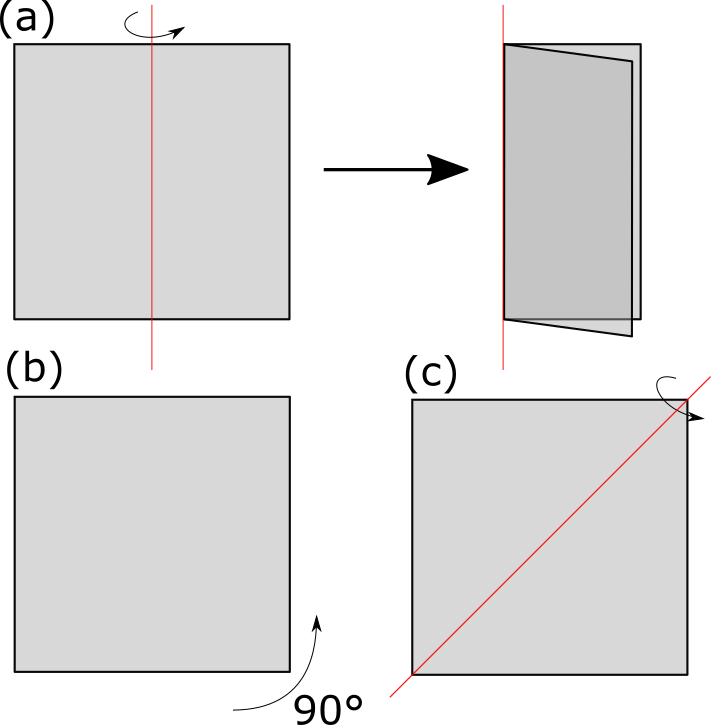
\includegraphics[width=0.7\columnwidth]{square_symmetry.png}
	\caption{正方形の対称性}
	\label{fig:square_symmetry}
\end{figure}

\begin{figure}[htbp]
	\centering
	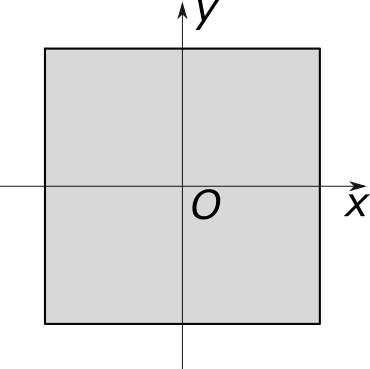
\includegraphics[width=0.4\columnwidth]{square_coordinate.png}
	\caption{正方形の座標系}
	\label{fig:square_coordinate}
\end{figure}

その他にも様々な対称性を、このような「ある変換に対する不変性」という形で定式化することができます。例えば、図\ref{fig:square_symmetry}(b),(c)はそれぞれ、正方形が90°回転、斜め方向の折り返しに関して不変である様子を表しています。これらも、それぞれ次のような変換に対応していると考えることができます。
\begin{align}
	C_4&: (x,y)\mapsto (y,-x)\\
	\sigma_d&: (x,y) \mapsto (y,x)
\end{align}

これらの変換はよく見るとすべて線形変換なので、行列を用いて表すことができます。例えば、
\begin{align}
	\sigma_x &= \mqty(-1 & 0 \\
					   0 & 1 ) \\
	C_4 &= \mqty(0 & 1 \\
				 -1& 0 )\\
	\sigma_d &= \mqty(0 & 1 \\
					1 & 0)
\end{align}
などです。これらの変換はすべて長さ(ノルム)を変えない直交変換になっていることにも注意してください。

さて、二つの変換を続けて行うことを、新しい一つの変換とみなせば、変換の合成を定義することができます。例えば、最初に$\sigma_x$という変換を行ってから、次に$C_4$という変換を行うことを$C_4 \circ \sigma_x$と書くことにしましょう。$C_4\circ \sigma_x$は、もちろん正方形を不変に保つ変換になっています。実際、先ほど導入した行列を用いて計算してみると、
\begin{align}
	C_4\circ \sigma_x &= 
	\mqty(	0	& 1 \\
		  	-1	& 0 )
	\mqty(	-1	& 0 \\
			0	& 1 ) = 
	\mqty(	0	& 1 \\
			1	& 0 ) = \sigma_d
\end{align}
となっていて、合成した結果もまた正方形を不変にする変換の一つになっていることが確かめられます。他にも、例えば$\sigma_y\circ\sigma_y$は、
\begin{align}
	\sigma_y\circ\sigma_y &= 
	\mqty(	1	& 0 \\
			0	& -1 ) 
	\mqty(	1	& 0 \\
			0	& -1 ) = \imat{2} 		 
\end{align}
と、単位行列になることがわかります。単位行列は、何もしない変換ですから、当然正方形は不変にする変換の一つということができます。一般に、このような何もしない変換のことを恒等変換と呼び、本記事では$E$と書くことにします。

\subsubsection{系の対称性を表す群}
ある注目する系について、前節で述べたような系を不変にする変換をすべて集めてきた集合$G$を考えましょう。この集合は、変換の合成を積とみれば群になっています。この場合の単位元は、恒等変換$E$になります\footnote{このあたりの「何を対称性の群の定義にするか」という話については、正直自分もよくわからないが、フォーマルには後述の「ハミルトニアンを不変にする変換全体の集合」というのが最も良いと思う。このように考えればきちんとこの集合が群になっていることも示すことができる。ただ、実際にモデルを作ったりするときは、始めに対称性の群がありきで、その対称性を持つようなハミルトニアンを考えたりする。まあ物理なので細かいことは気にしない。}。



\end{document}